\author{Sylvain Kahane and Kim Gerdes}
\title{Syntaxe théorique et formelle}
\subtitle{Volume 1 : Modélisation, unités, structures}
\renewcommand{\lsSeries}{tbls}
\renewcommand{\lsSeriesNumber}{9}
\renewcommand{\lsID}{241}
\BookDOI{10.5281/zenodo.6446068}
\ISBNdigital{978-3-96110-341-6}
\ISBNhardcover{978-3-98554-037-2}
\BackBody{Conçu comme une introduction générale à la syntaxe, cet ouvrage présente les notions de base nécessaires à une étude de la combinaison des unités lexicales et grammaticales au sein d’un énoncé. Sans se placer dans un cadre préconçu, l’ouvrage étudie les différentes possibilités pour la représentation des structures syntaxiques, en fonction des principes généraux et des critères particuliers retenus.

Élaboré avec l’objectif de fournir une base pour l’enseignement de la syntaxe à l’université, cet ouvrage souhaite montrer qu’on peut dégager de manière méthodique les propriétés des langues et mettre de l’ordre dans la forêt vierge que constitue chaque langue. Il est divisé en trois parties : comment élaborer le modèle d’une langue, comment déterminer les unités de base de la langue en fonction de leur sens, forme et combinatoire, comment définir et représenter les différents modes d’organisation des unités. Cette dernière partie présente une abondance de diagrammes syntaxiques de diverses natures.

L’ouvrage est découpé en de petites sections, alternant le contenu principal avec des éclairages, des notes historiques, des élaborations plus formelles, des exemples linguistiques dans diverses langues, des propositions de lectures additionnelles et des exercices avec des éléments de correction.}

\proofreader{Guillaume Jacques, Sebastian Nordhoff}
\dedication{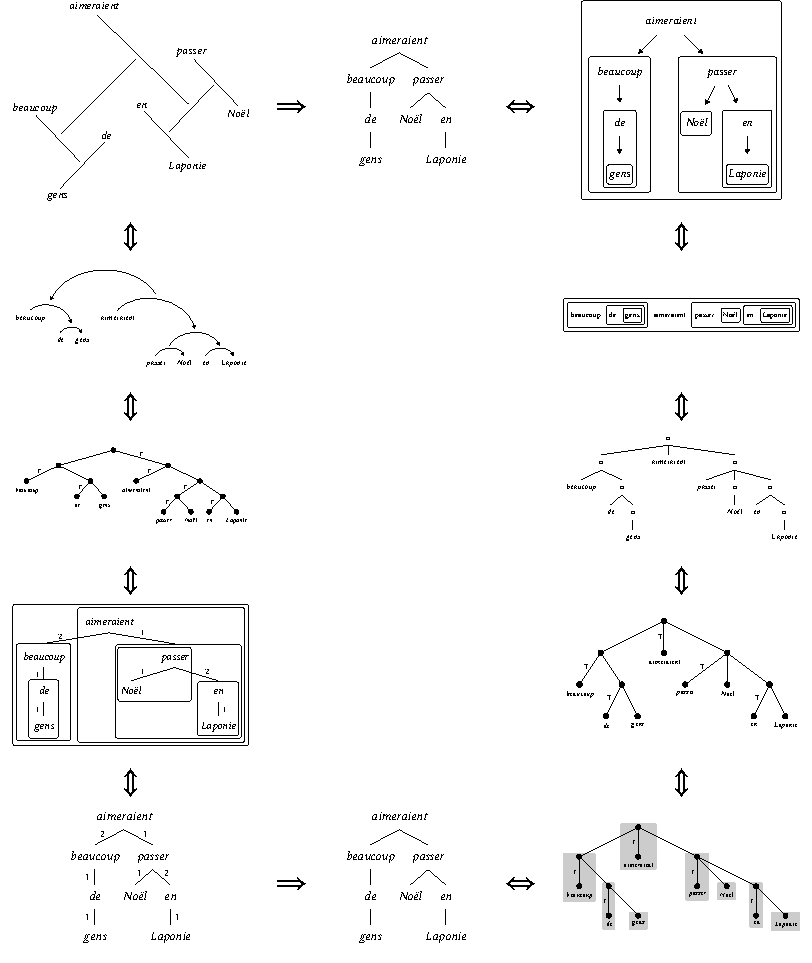
\includegraphics[width=\textwidth]{figures/graphs-collection.pdf}}
